\documentclass[11pt,a4paper]{article}
\usepackage[margin=24mm,headheight=14pt]{geometry}
\usepackage{fontspec}
\setmainfont{Latin Modern Roman}
\usepackage{amsmath,amssymb,amsthm,mathtools,unicode-math}
\setmathfont{Latin Modern Math}
\usepackage{microtype,booktabs,array,enumitem,xcolor,fancyhdr,xurl,tikz}
\usetikzlibrary{arrows.meta}
\usepackage[colorlinks,linkcolor=blue!45!black,urlcolor=blue!45!black,
 citecolor=blue!45!black]{hyperref}
\hypersetup{pdftitle={RH and Dirichlet GRH: a short mathematical guide}}
\setlength{\parskip}{3pt}
\setlength{\emergencystretch}{2em}
\setlist{topsep=3pt,itemsep=3pt,parsep=0pt}
\pagestyle{fancy}
\fancyhf{}
\fancyhead[L]{\small RH and Dirichlet GRH}
\fancyhead[R]{\small A mathematical guide}
\fancyfoot[C]{\thepage}
\newtheorem{theorem}{Theorem}[section]
\newtheorem{lemma}[theorem]{Lemma}
\newtheorem{proposition}[theorem]{Proposition}
\DeclareMathOperator{\Rea}{Re}
\DeclareMathOperator{\covol}{covol}
\DeclareMathOperator{\rk}{rk}
\newcommand{\R}{\mathbb R}
\newcommand{\C}{\mathbb C}
\newcommand{\Z}{\mathbb Z}
\newcommand{\Q}{\mathbb Q}
\title{RH and Dirichlet GRH\\[3pt]\large A short mathematical guide}
\author{}
\date{21 November 2026}
\begin{document}
\maketitle
\vspace{-1.8em}
\begin{abstract}
The purpose of this guide is to explain the problem and the proposed proof
in a small number of steps. The analytic reductions below are proved;
several arithmetic inputs are supplied by classical theorems. The central
arithmetic construction is still incomplete in this reconstruction.
In particular, this is a guide to a proof program, not a completed proof
of the Riemann hypothesis. It explains what becomes simpler when only
the ordinary Riemann hypothesis is sought, and where the difficulty survives.
Detailed arguments are in the accompanying manuscript~\cite{reconstruction}.
\end{abstract}

\section{The two questions}

For a complex number $s$ with real part greater than one, the Riemann
zeta function is
\[
 \zeta(s)=\sum_{n=1}^{\infty}n^{-s}
         =\prod_{p\ \mathrm{prime}}(1-p^{-s})^{-1}.
\]
The equality connects addition over integers with multiplication over
primes. Analytic continuation extends $\zeta$ to the complex plane,
with a simple pole at $s=1$. Its nontrivial zeros lie in
$0<\Rea s<1$ and are reflected across the line $\Rea s=1/2$.
The \emph{Riemann hypothesis}, or RH, says that every such zero lies on
that line~\cite{dlmf}.

A Dirichlet character modulo $q$ is a homomorphism from
$(\Z/q\Z)^\times$ to the unit circle, extended by zero on integers
not coprime to $q$. It gives the function
\[
 L(s,\chi)=\sum_{n=1}^{\infty}\frac{\chi(n)}{n^s}
 =\prod_p(1-\chi(p)p^{-s})^{-1}\qquad(\Rea s>1).
\]
Dirichlet GRH asks for the same zero statement for all these functions.
The conductor-one character gives $\zeta$. A character is primitive when
it is not induced from a smaller modulus. The general case reduces to
primitive characters, since the extra Euler factors have no zeros in
$\Rea s>0$~\cite{dlmf}.

RH therefore has one analytic target; Dirichlet GRH has a family of
targets. An auxiliary character used to prove RH is not an additional
target unless the argument requires its own zero statement.

\section{A prime sum that detects zeros}

Let $\Lambda(n)=\log p$ when $n$ is a positive power of a prime $p$,
and let $\Lambda(n)=0$ otherwise. Write $\gamma$ for Euler's constant.
For $x\ge1$ define
\begin{equation}\label{gdef}
 G(x)=\sum_{n\le x}\Lambda(n)(x/n-1)-x\log x+(1+\gamma)x.
\end{equation}
The factor $x/n-1$ makes a smoothed sum: a newly entering term has
weight zero. The last two terms remove the contribution of the pole
of $\zeta$ at one. Thus $G$ measures the fluctuation left after that
main contribution is removed.

The useful relation is an exact integral identity. For $\Rea s>1$,
\begin{equation}\label{mellin}
 \int_1^\infty G(x)x^{-s-1}\,dx
 =-\frac{\zeta'(s)/\zeta(s)}{s(s-1)}
  -\frac1{(s-1)^2}+\frac{1+\gamma}{s-1}.
\end{equation}
Indeed,
\[
 \int_n^\infty(x/n-1)x^{-s-1}\,dx
       =\frac{n^{-s}}{s(s-1)},\qquad
 \sum_n\Lambda(n)n^{-s}=-\frac{\zeta'(s)}{\zeta(s)}.
\]
Absolute convergence justifies the interchange. The apparent singularity
of~\eqref{mellin} at one is removable. A zero $\rho$ of multiplicity $m$
in the critical strip gives a genuine pole with residue
\begin{equation}\label{residue}
                         -\frac{m}{\rho(\rho-1)}.
\end{equation}
This is the basic bridge: a sufficiently small prime-sum fluctuation
leaves no room for a zero to the right of one half.

For a primitive nonprincipal character, the analogous corrected sum is
\[
 G_\chi(x)=\sum_{n\le x}\Lambda(n)\chi(n)(x/n-1)
             +x\frac{L'(1,\chi)}{L(1,\chi)}.
\]
We use the classical nonvanishing $L(1,\chi)\ne0$. Its Mellin transform
has exactly the residue~\eqref{residue} at a zero of $L(s,\chi)$.
Put $G_1=G$ for the conductor-one character.

\section{A particularly short analytic route for RH}

The following theorem isolates an RH-only problem with a short proof.
It requires a bound for every sufficiently large $x$. A later section
gives a more flexible interval version used by the arithmetic construction.

\begin{theorem}[One-sided zeta criterion]\label{rhcriterion}
Suppose that for every $\delta>0$ there are finite constants
$C_\delta\ge0$ and $X_\delta\ge1$ such that
\[
             G(x)\le C_\delta x^{1/2+\delta}
                         \qquad(x\ge X_\delta).
\]
Then RH holds. No lower bound for $G$ is needed.
\end{theorem}

Here is a self-contained form of the positivity principle used in its proof.

\begin{lemma}[Positivity and the convergence boundary]\label{landau}
Let $f\ge0$ be locally integrable on $[X,\infty)$, where $X\ge1$, and
suppose its Mellin integral converges for all sufficiently large real $s$.
If that integral has a holomorphic continuation to a neighborhood of
each real $s>\theta$, its abscissa of convergence is at most $\theta$.
\end{lemma}

\begin{proof}
Suppose the finite abscissa is $\sigma_c>\theta$. Holomorphy near
$\sigma_c$ gives a real $a>\sigma_c$ and a Taylor radius $R>a-\sigma_c$.
For $0<t<R$, the Taylor series at $a$ has the form
\[
 F(a-t)=\sum_{k\ge0}\frac{t^k}{k!}
             \int_X^\infty f(x)(\log x)^k x^{-a-1}\,dx.
\]
All integrands are nonnegative. Tonelli's theorem makes the right side
equal to
\[
                  \int_X^\infty f(x)x^{-(a-t)-1}\,dx.
\]
Choosing
$a-\sigma_c<t<R$ contradicts the definition of $\sigma_c$.
The case of abscissa $-\infty$ already satisfies the conclusion.
\end{proof}

\begin{proof}[Proof of Theorem~\ref{rhcriterion}]
Fix $\theta=1/2+\delta<1$ and put
$f(x)=C_\delta x^\theta-G(x)$ for $x\ge X_\delta$. It is nonnegative.
The elementary estimate $|G(x)|\ll x(1+\log^2x)$ gives initial
convergence. Formula~\eqref{mellin}, after subtracting an integral over
a finite interval, continues its Mellin transform.

There is no real obstruction above $\theta$. For $s>1$ the zeta function
is positive. For $0<s<1$ the alternating series
\[
 \eta(s)=\sum_{n\ge1}(-1)^{n-1}n^{-s}>0,
 \qquad \zeta(s)=\frac{\eta(s)}{1-2^{1-s}}<0
\]
proves real nonvanishing; grouping consecutive terms proves the positivity.
The singularity at one in~\eqref{mellin} was removed. The new term
$C_\delta X_\delta^{\theta-s}/(s-\theta)$ has its only real pole at
$\theta$. Lemma~\ref{landau} therefore gives convergence, and hence
holomorphy of the integral, on $\Rea s>\theta$.

A zero of $\zeta$ there would give the nonzero residue~\eqref{residue},
which is impossible. Let $\delta$ tend to zero. Reflection by the
functional equation excludes zeros to the left of one half as well.
\end{proof}

The proof of this implication is complete. Establishing its prime-sum
hypothesis remains the arithmetic problem. Neither the prime number
theorem nor a fixed zero-free region reaching only to some
$\theta>1/2$ supplies that hypothesis.

For zeta, the same proof also works from an eventual lower bound
$G(x)\ge-C_\delta x^{1/2+\delta}$: take
$f=C_\delta x^{1/2+\delta}+G$ instead. Either direction may be chosen
at each accuracy. Real nonvanishing of zeta is essential to this argument.

\section{The more flexible analytic target}

The arithmetic construction need not control every sufficiently large
real number. It is enough to control whole intervals $[Y,Y^b]$ for
arbitrarily large $Y$, with $b>1$ fixed during each limiting argument.
Such an interval has logarithmic length $(b-1)\log Y$, which tends to
infinity; control at isolated large values of $x$ does not suffice.

One can also retain auxiliary characters with positive coefficients.
For each positive integer $j$, let
\[
 H_j(x)=\sum_{\nu\in\mathcal C_j}a_{j,\nu}\Rea G_\nu(x),
                       \qquad a_{j,\nu}>0,
\]
where $\mathcal C_j$ is finite. For RH, require that the conductor-one
character occurs. For a specified Dirichlet $L$-function, require its
primitive character or its conjugate to occur. The completed interval
criterion in the full manuscript says that
\begin{equation}\label{window}
 H_j(x)\le M_j x^{1/2+\delta_j}\quad(Y\le x\le Y^{b_j}),
 \qquad \delta_j>0,\quad\delta_j\longrightarrow0,
\end{equation}
on arbitrarily late such whole intervals excludes every off-line zero
of the retained target~\cite{reconstruction}. Here $0\le M_j<\infty$,
$b_j>1$, the auxiliary characters and their weights may depend on $j$.
They are fixed while the intervals for that $j$ go to infinity.

The reason positive coefficients are useful is exact. At a zero $\rho$,
the residue of the transform of $H_j$ is
\[
 -\frac1{\rho(\rho-1)}
   \sum_{\nu\in\mathcal C_j}\frac{a_{j,\nu}}2
       \bigl(m_\nu(\rho)+m_{\bar\nu}(\rho)\bigr).
\]
Every multiplicity is nonnegative. A zero of a retained target gives
a nonzero sum, so the auxiliary terms cannot cancel its pole.
The interval argument is longer than Lemma~\ref{landau}, but allows
a weaker arithmetic premise. Its complete proof is kept in the
full manuscript.

\section{How arithmetic is meant to bound the prime sum}

The construction compares two kinds of size for the same integral maps.
Divisibility at finite primes makes an integral image small in an
arithmetic sense. Norm estimates at the complex embeddings constrain
the corresponding real volumes. A slope comparison combines the two.
An integral transform called a theta lift supplies the candidate maps.
Its definition, periods and measures matter: both estimates must concern
that actual map with those same normalizations.

\subsection*{Volumes, degrees and exceptional subspaces}

For clarity, consider first a Euclidean lattice $L$ over $\Z$.
Its covolume is the volume of a fundamental parallelepiped. Define
\[
 \deg L=-\log\covol L,\qquad
 \mu(L)=\frac{\deg L}{\rk L}.
\]
The slope $\mu$ is the logarithmic size per dimension. Lattices over
number fields use the corresponding normalized arithmetic degree.

Suppose an orthogonal rational projection $P$ satisfies $NP(L)\subset L$
for an integer $N\ge1$. Put
\[
 L_+=L\cap\operatorname{im}P,\quad
 L_-=L\cap\ker P,\quad
 g=\rk L_+>0,\quad b=\rk L_-,\quad r=g+b.
\]
Writing $I=[L:L_+\oplus L_-]$, one has the exact identity and bound
\begin{equation}\label{cut}
 g\mu(L_+)=r\mu(L)-b\mu(L_-)-\log I,
                   \qquad I\le N^{\min(g,b)}.
\end{equation}
Orthogonality gives the covolume identity. The quotient of $L$ by
$L_+\oplus L_-$ embeds both in $N^{-1}L_+/L_+$ and in
$N^{-1}L_-/L_-$, giving the index bound. When $b=0$, the discarded
term is omitted and $I=1$.

Thus a lower slope bound for $L$ gives one for $L_+$ once the actual
discarded degree and the integral index are controlled. Small discarded
dimension alone is insufficient: its mean slope could be very large.
An exponential estimate for the discarded fraction is one possible
supplier, but suitable polynomial decay also suffices when the other
terms have appropriately smaller growth.

The missing geometric input is a bound for the specific lattice of
cuspidal sections with its prescribed periods and metric. A general
lattice identity such as~\eqref{cut} does not construct that lattice
or prove its initial lower slope.

The component calculation can now be stated with two averaged height
bounds. For its actual positive component weights $w_Z$, put
\[
 \overline h=\frac{\sum_Zw_Zh_Z}{\sum_Zw_Z},\qquad
 h_- =\frac{\sum_Zw_Z\max(-h_Z,0)}{\sum_Zw_Z}.
\]
A lower bound for $\overline h$ and an upper bound for $h_-$ suffice for
the refined component estimate, once the stated section remainders
are controlled. A separate lower height bound for every component is
stronger than necessary. Negative heights cannot be hidden by a large
positive average: their actual weighted contribution is retained.
Descent from a covering also keeps the exact rank ratio and section
error, avoiding an unnecessary doubling of that error.

\subsection*{Average the losses before bounding them}

For a finite abelian group and a subgroup $B$, character orthogonality gives
\[
 \frac1{|B|}\sum_{u\in B}\psi(u)
 =\begin{cases}1,&\psi|_B=1,\\0,&\psi|_B\ne1.\end{cases}
\]
This removes unwanted character contributions exactly. Applying it to
the arithmetic comparison gives an inequality of the form
\begin{equation}\label{average}
 H(x)\le R_{\mathrm{proj}}(x)
       +\frac{2\bigl(\overline E(x)+R_{\mathrm{trans}}(x)\bigr)}
                    {n_T m b_0 d_0}.
\end{equation}
Here $n_T$ counts the chosen labels, $m$ counts the maps,
$b_0>0$ is the common weight scale, and $d_0>0$ is the selected density.
The quantity $\overline E$ is the arithmetic discrepancy averaged over
translations. The two
remainders are explicit finite sums: one measures the error in the
chosen character projection, the other the replacement of the original
weights by their principal values. The full statement defines every
term and proves~\eqref{average}~\cite{reconstruction}.

Only an upper bound for the total normalized loss is needed. Negative
discrepancies may cancel positive ones. The same principle improves the
comparison of the complex frames defining the map norms: average their
actual errors before estimating the nonlinear terms. This retains the
correlation between a frame's error, its source slope spread and its
target height gap. It can cost much less than a common worst-case bound,
but the required moments still concern the same maps and metrics.

\section{The preferred proof structure}

Three groups of input feed the arithmetic comparison.

\begin{enumerate}
\item \textbf{Arithmetic selection and cohomology.}
Choose the auxiliary characters and levels, then control the relevant
cohomological errors. Algebraic $K$-theory supplies a shorter route to
the coarse bound. Some integral and complementary-parity bounds remain.
\item \textbf{Integral maps and analytic norms.}
Construct nonzero theta maps, establish their finite-prime divisibility,
and bound their archimedean norms. Local positivity and several exact
identities are proved; the required global estimates in growing
dimensions are still being assembled.
\item \textbf{Geometric degrees.}
Identify the lattice with its prescribed metric, prove its lower slope,
and control the discarded-degree and index terms in~\eqref{cut}.
\end{enumerate}

Classical theorems now supply the required Galois representations~\cite{blggt}.
Their weights, local correspondences
and period normalizations have been compared with the required data.
The separate construction of those representations by stable theta
lifting can therefore be omitted from the preferred argument. Theta
identities and geometric estimates used elsewhere retain their own roles.

\begin{center}
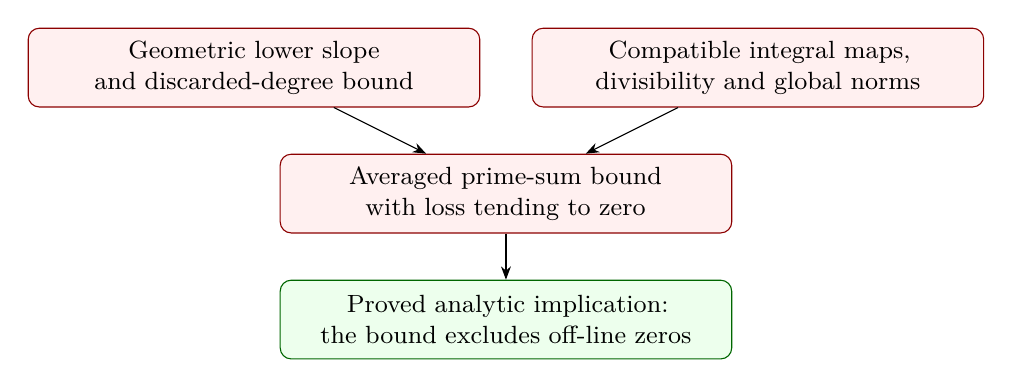
\begin{tikzpicture}[>=Stealth,
 every node/.style={draw,rounded corners,align=center,font=\small,
                   text width=5.5cm,minimum height=1cm},
 open/.style={fill=red!6,draw=red!55!black},
 proved/.style={fill=green!7,draw=green!40!black}]
 \node[open] (geom) at (-3.2,0) {Geometric lower slope\\and discarded-degree bound};
 \node[open] (maps) at (3.2,0) {Compatible integral maps,\\divisibility and global norms};
 \node[open] (budget) at (0,-1.6) {Averaged prime-sum bound\\with loss tending to zero};
 \node[proved] (criterion) at (0,-3.2) {Proved analytic implication:\\the bound excludes off-line zeros};
 \draw[->] (geom)--(budget);
 \draw[->] (maps)--(budget);
 \draw[->] (budget)--(criterion);
\end{tikzpicture}
\end{center}
Red boxes are unresolved mathematical obligations. The green implication
is proved under its stated premise. All the arithmetic and geometric
objects entering a box must be compatible; separately chosen objects
with unrelated good estimates cannot be combined.

\section{What becomes simpler for ordinary RH?}

The analytic target becomes just $G$. Theorem~\ref{rhcriterion} uses
only zeta, its functional equation and positivity. The arithmetic
comparison still needs auxiliary characters and growing spaces.

\subsection*{A positive kernel removes the symmetry requirement}

Partition the actual archimedean weights into thick and thin places.
The thick weights lie in $[b_0,b_0+r]$, where $r$ is small compared with
$b_0$. Instead of making all weight distributions invariant, compare
only the thick weights with their common lower endpoint $b_0$.

The crucial fact is positivity. At each prime power, the complete
character sum in the arithmetic identity is a nonnegative residue-class
count, including at ramified primes. Its contribution as a function of
a weight is a sum of nonnegative multiples of
\[
                           (a/n-w)_+,
                 \qquad z_+=\max(z,0),
\]
together with $a\log w$ and a constant. Moving a thick weight upward
from $b_0$ therefore has a controlled one-sided cost. The constants
involving logarithmic derivatives cancel from this difference.
Sum over translations before taking absolute values: the normalized
cost then has neither a field-degree factor nor an inverse-density
factor. These are proved algebraic cancellations, not assumptions
about independence of the weights~\cite{reconstruction}.

The thin weights are smaller, so their arguments $a/w$ are much larger.
The existing uniform quasi-RH estimate controls these samples. It still
concerns the full auxiliary character family; four characters suffice
only for the remaining main-scale expression.

\subsection*{One averaged arithmetic discrepancy remains}

After the thick weights are fixed and translations averaged, the
main-scale expression is
\[
 G+G_{\chi_q}-G_{\chi_d}-G_{\chi_q\chi_d}
                         =G-C_{q,d},\qquad
 C_{q,d}=G_{\chi_d}+G_{\chi_q\chi_d}-G_{\chi_q},
\]
where $\chi_q,\chi_d$ are the quadratic characters of the two distinct
auxiliary prime conductors. Their signs come from character
orthogonality. The trivial coefficient is $1$ and one quadratic
coefficient is always $-1$; the total coefficient is zero. Thus these
projections alone cannot produce a positive multiple of zeta.
Only an upper bound for the single signed companion $C_{q,d}$ is needed.

Let $n_T$ be the number of top labels and put
$k=n_Tmb_0d_0/2>0$, using the same normalization as~\eqref{average}.
Under the stated size conditions, $|a_t/b_0-x|\le1$ and
$d_0\ge x^{-\varepsilon}$, the preceding comparison gives
\begin{equation}\label{rhbudget}
 G(x)\le\frac{\overline E(x)}k
       +\frac1{n_T}\sum_t C_{q,d}(a_t/b_0)
       +O\!\left((1+\log x)^2+x^{-1+\varepsilon}\right).
\end{equation}
Here the thin-sample bound uses the uniform quasi-RH premise, and the
constant is fixed at each accuracy before $x$ grows. The full proof
retains the explicit error constants. Centering only the zeta term
at $x$ costs the logarithmic error; no nonprincipal derivative bound
is needed for that step.

The simultaneous quadratic selection supplies a square-root-scale
bound for the companion under the same uniform premise, on intervals
containing all the samples. The next task is therefore to bound the
normalized discrepancy $\overline E/k$, or its sum with the signed
companion, for one compatible arithmetic and geometric construction.
The auxiliary primes may vary with $x$, since the analytic target in
\eqref{rhbudget} is always the same zeta sum. The estimate must hold
on whole intervals as in~\eqref{window}, with exponent loss tending
to zero; isolated favorable values do not suffice.

\begin{center}
\begin{tabular}{@{}p{.39\linewidth}p{.54\linewidth}@{}}
\toprule
Simplification for RH & Consequence \\
\midrule
One analytic target & The short zeta criterion applies. \\
Only four main-scale characters & One signed quadratic companion
remains. \\
Thick weights fixed before averaging & Symmetry is unnecessary. \\
Thin samples at large arguments & Uniform quasi-RH controls them. \\
One averaged discrepancy & Combine geometric and map bounds. \\
\bottomrule
\end{tabular}
\end{center}

This gives a shorter proved reduction for RH. A much shorter complete
proof has not yet been obtained: the nonzero integral maps and the
uniform arithmetic and geometric estimate still have to be supplied.

\section{How the newer zero-free results help}

A uniform zero-free half-plane $\Rea s>\vartheta$, with
$1/2<\vartheta<1$, helps select the moving quadratic companions and
bounds the thin samples at their much larger arguments. The required
uniformity includes the conductors of the auxiliary family. A statement
for each fixed character with uncontrolled constants would not suffice.
When this same hypothesis excludes a real exceptional zero, a separate
exclusion of that zero is unnecessary.

These inputs do not by themselves make $\delta_j$ in~\eqref{window}
tend to zero. Excluding real exceptional zeros is also a different
assertion from excluding every nonreal zero to the right of one half.
For the zeta-only proof above, real nonvanishing follows directly
from the alternating series. If quadratic auxiliary functions remain
in the arithmetic construction, their own estimates must still be supplied.

The next mathematical task is to produce compatible data for which
the right side of~\eqref{rhbudget} meets the interval criterion
\eqref{window}. The two geometric height moments, actual section
remainders, discarded degrees and integral indices, nonvanishing and
divisibility of the maps, and global norm estimates are concrete parts
of that task. Their combined normalized loss must tend to zero in
exponent. The more general Dirichlet target retains its additional
character quantifiers; its finite-error comparison is~\eqref{average}.

\begin{thebibliography}{9}
\bibitem{dlmf}
NIST Digital Library of Mathematical Functions,
\S\S25.2, 25.4, 25.10 and 25.15: the zeta and Dirichlet $L$-functions,
their functional equations and zeros.
\url{https://dlmf.nist.gov/25}.

\bibitem{reconstruction}
\href{https://github.com/JoseBrox/GRH_distillation/blob/main/paper/main.pdf}
{\emph{Analytic and arithmetic reductions toward Dirichlet GRH}},
the accompanying mathematical reconstruction.

\bibitem{blggt}
T. Barnet-Lamb, T. Gee, D. Geraghty and R. Taylor,
\emph{Potential automorphy and change of weight},
Annals of Mathematics \textbf{179} (2014), 501--609, Theorem 2.1.1;
and \emph{Local-global compatibility for $l=p$, II},
Annales scientifiques de l'\'Ecole normale sup\'erieure
\textbf{47} (2014), 165--179, Theorem 1.1.

\bibitem{announcement}
L. Alp\"oge, \href{https://alpo.ge/remark.pdf}
{announcement of a proof of RH and Dirichlet GRH}, 20 November 2026.
\end{thebibliography}
\end{document}
